\section{Valg af tonearter}
\subsection{Hvorfor er tonearten vigtig?}
På mange måder er kunsten i at lave revy, at optimere under begrænsninger.
Det måske klareste eksempel på dette er valget af tonearter til sange.
Det klareste mål er, at sangernes stemmer klinger godt i den valgte toneart. Dette kan i sig selv være svært at opnå, idet der typisk er flere sangere på hver sang, der hver har forskellige områder hvor de klinger godt. For nogle er dette område endda relativt snævert.
Men der er mange musikalske elementer hvis kvalitete afhænger meget af toneart. Herunder er et par eksempler:
\begin{itemize}
    \item Basgange der er melodiske er følsomme overfor større transponeringer; Hvis de bliver for høje kan de ikke mærkes, og hvis de bliver for dybe kan de ikke høres. Hvis motivet/linien bliver knækket over en oktav mister det sin melodiske karakter. Prøv f.eks. at spille Lizzo's Juice i Gm eller G\#m.
    \item Blæsere har på samme måde som sangere bestemte registre hvor de klinger bedst. Derfor kan blæserarrangementer der lyder godt in én toneart, nemt komme til at lyde skidt i en anden, hvis de trantponeres naivt. Derudover kan nogle tonearter have væsentligt sværere greb end andre. Også instrumenternes intonation er påvirket af toneart og register. 
    \item Guitarriffs har samme grundlæggende problem som baslinier; de er skrevet til at have bestemte centrale toner i bunden af registeret. Derudover gøres der ofte brug af åbne strenge på en måde der gør dem svære at spille i andre tonearter.
    \item Harmoniers karakter ændres, hvis registeret ændres. Generelt vil harmonier lyde mindre klare, desto lavere register de spilles i, så hvilke voicings der er mulige (eller behagelige) afhænger af tonearten.
\end{itemize}

Derudover vil man selvfølgelig gerne undgå at ændre toneart på sangene undervejs i processen. Medmindre bandet er virkelig godt, vil det forårsage en del merarbejde og forøge risikoen for fejl.

\subsection{Hvad er en god toneart?}
På baggrund af betragtingerne i sidste afsnig, vil jeg opstille følgende kriterier for at en toneart er godt valgt i revyregi:
\begin{enumerate}
    \item Sangerne klinger godt
    \item Centrale musikalske elementer fungerer godt
    \item Der er ikke behov for at ændre toneart undervejs
\end{enumerate}
Hvilke musikalske elementer der er centrale er selvfølgelig en vurderingssag, og hvor godt de kan fungere i forskelliger tonearter kræver nok noget erfaring, samt kendskab til sit band. Men hvis du er blevet valgt til bandboss, er det nok fordi dine medrevyster stoler på din musikalitet og dømmekraft (:

Under alle omstændigheder kræver det et godt samarbejde mellem bandboss og sangboss at sætte tonearterne godt.

I det følgende afsnit vil jeg beskrive en nem og en mere omfatternde måde at vælge tonearter til sine revysange. Jeg vil også prøve at overbevise dig om, at den mere omfattende metode er besværet værd.

\subsection{Optimalt valg af tonearter}
Når man sætter tonearter på den nemme måde, lader man først manusgruppe og/eller instruktører og/eller koordinatorer fordele sangrollerne på sangerne. Herfra finder bandet i samarbejde med sangboss og sangerne på hver sang en toneart der fungerer for sangerne på sangen. I denne model er band først involveret i processen efter rollerne er fordelt. Det kræver derfor mindre af bandboss tidligt i revy-processen.

Man havner dog nemt i uløselige dillemaer hvor noget må give og det er altid ærgerligt.

\subsubsection{En mere omfattende metode}
I min optik kræver et optimalt valg af tonearter, at bandbossen og sangbossen er med til at fordele roller.

Sangbossens rolle er at have lavet foresyngning/tonelejetest med alle sangere, så hen har et klart indtryk af deres range. Denne information skal gerne være indtastet i et skema, så det er nemt tilgængeligt og overskueligt.

Bandbossens rolle er, at have et skema, hvor der for hver sang er noteret spændet for melodien af hvert stykke (vers, omkvæd osv).
Derudover skal bandbossen have et overblik over de vigtigste musikalske elementer i hver sang, som potentielt kan påvirkes af tonearten.
På den måde kan bandboss og sangboss komme med forslag til rollefordeling, som vil formindske mængden af toneart-relaterede problemereller blot give input til en given sangerbemanding.
Det åbner også muligheden for at tildele sangere specifikke stykker af sangen eller specifikke roller/stemmer. Dette gør det markant nemmere at få alle hensyn til at gå op. Se figur 1 for et eksempel på et skema med spænd af melodi.
%TODO: Indsæt eksempel på skema her
\begin{figure}
    \centering
    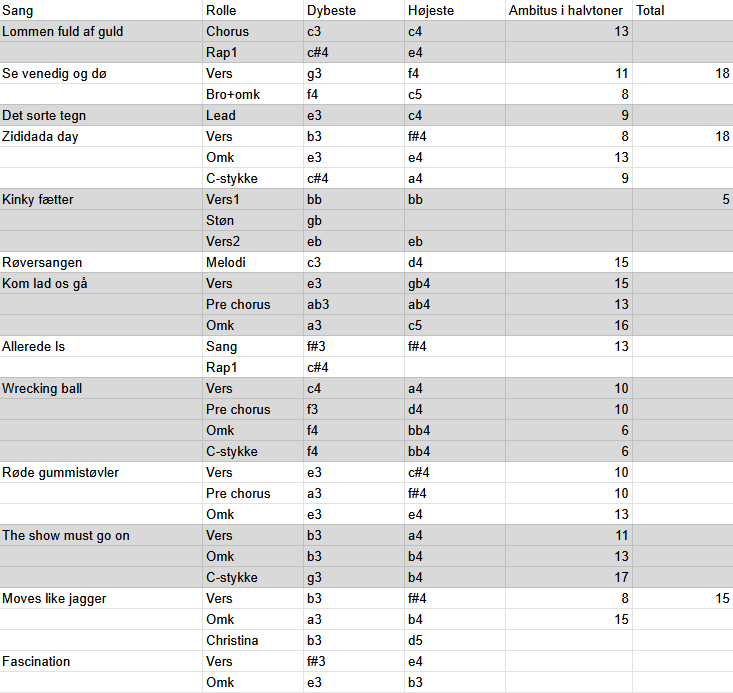
\includegraphics[width=1.1\linewidth]{satyr-2021-sangroller-ambitus.png}
    \caption{Eksempel på oversigt over ambitus for hver sektion af hver sang, i originaltoneart. Fra SaTyR 2021.}
    \label{fig:ambitus-oversigt}
\end{figure}

Som band er det klart at rollefordeling der tager hensyn til diverse toneart-betragtninger kan komme mange problemer i forkøbet og spare meget hovedpine. Som sangboss bliver ens job nok også en del sjovere, idet man ikke behøver bruge ligeså meget energi på "elementære" problemer.

Jeg vil dog også mene at dette er til fordel for sangerne, særligt de mindre trænede. Det er åbenlyst nemmere at synge godt når ens stemme ligger godt til en, men det er også meget tryggere. Det, at føle sig sikker på, at man kan ramme og nå tonerne er kritisk for svagere sangere. Det er et generelt problem for utrænede sangere at de ikke tør synge igennem, og det gør alle dele af processen meget vanskeligere. Dette problem kan i høj grad kommes til livs, ved at tildele dem opgaver som de oplever, at de ved de kan bære.
I sidste ende er det også afgørende for at sangerne får en god oplevelse med at synge på scenen.
Publikum vil også sætte pris på det, omend de ikke ved hvad alternativet havde været.
